\documentclass[a4paper,11pt]{article}
\usepackage[a4paper, total={6in, 8in}]{geometry}
\usepackage[T1]{fontenc}
\usepackage[utf8]{inputenc}
\usepackage[english,serbian]{babel}
\usepackage{graphicx}
\usepackage{subfig}
\usepackage{fancyhdr}

\renewcommand{\figurename}{Slika}
\graphicspath{ {./img/} }

\title{Smerač}
\author{Aleksa Siriški}
\date{Novembar 2022}

\begin{document}

\pagestyle{empty}
\begin{center}
    \begin{figure}
        \centering
        
\includegraphics[height=3cm,width=3cm]{pmf}
    \end{figure}

    \textbf{
    UNIVERZITET U NOVOM SADU
    \\
    PRIRODNO-MATEMATIČKI
    \\
    FAKULTET
    \\
    DEPARTMAN ZA MATEMATIKU
    \\
    I INFORMATIKU
    }

\end{center}
\vfill
\begin{center}
	\begin{huge}
		\textbf{Smerač}
		\bigskip 
	\end{huge}
	\\
	\begin{large}
        \textbf{- seminarski rad iz predmeta Skript jezici -}
	\end{large}
\end{center}
\vfill
\begin{center}
    Aleksa Siriški, 159/22
    \\
    Novi Sad, 2022.
\end{center}
\newpage

\pagestyle{plain}
\renewcommand{\contentsname}{Sadržaj}
\addcontentsline{toc}{section}{Sadržaj}
\tableofcontents
\newpage

\pagestyle{fancy}
\fancyhf{}
\lhead{Smerač}
\rhead{Aleksa Siriški}
\cfoot{\thepage}

\section{Uvod}
\subsection{Discord}
Discord\cite{discord}, kao jedna od najpopularnijih društvenih mreža za programere i entuzijaste računarskih tehnologija, je logičan izbor za razmenu informacija i raspoređivanje časova IT i RN smerova Univerziteta u Novom Sadu. Uprkos jednostavnosti Discord-ovog grafičkog interfejsa nije lako omogućiti studentima da sami sebi određuju smer a integracija sa Google kalendarom je apsolutno neizvodljiva. Na sreću, Discord tim je osposobio trećim licima da lako kreiraju 'Bot' naloge i uz pomoć njihovog REST api će nastati Smerač - Discord Bot stvoren da omogući studentima izbor sopstvenog smera kao i integraciju Google kalendara u prostom Discord chat-u.
\subsection{Python}
Smerač je Python\cite{python} skripta napisana u svega 400 linija koda. Računajući da korisnicima nije bitno da li će im smer biti dodeljen za 1ms ili 1s Python je bio prikladan izvor. Najpre zbog mnogobrojnih ugrađenih biblioteka i modula, kao što su discordpy\cite{discordpy} i asyncio, ali i zbog jednostavne sintakse koja je omogućila eksponencijalan razvoj ovog programa.
\subsection{Ideja}
Discord bot koji mora biti dovoljno jednostavan ali isto tako i univerzalno programiran da se može lako primeniti na više različitih okruženja (Discord servera). Takva prilagodljivost se postiže pametnim planiranjem toka rada programa i korišćenjem promenljivih okruženja (eng. \textit{environment variables}). Takođe je jako bitna licenca koja će se koristiti, da ne bi došlo do krađe autorskih prava i zloupotrebe softvera. Tačno iz tih razloga odabrana licenca za Smerač će biti GNU General Public License\cite{gpl}.
\subsection{Asinhronizacija}
Kako bi program mogao da istovremeno čita poruke od različitih korisnika potrebno je kreiranje dodatnih niti. Pomoću biblioteke asyncio\cite{asyncio} Smerač će imati mogućnost paralelnog parsiranja kalendara i dodeljivanja smera svakom studentu koji to zatraži. Pored bržeg izvođenja programa asinhrone funkcije služe da oduzmu čekanje odgovora od servera, tj. ako zahtev prvog korisnika traje duže da se obradi drugi korisnici ne moraju da čekaju prvog da dobije odgovor nego se i njihovi zahtevi takođe obrađuju u istom trenutku.
\subsection{Smerovi}
Najbitnija a najjednostavnija funkcionalnost Smerača će biti dodeljivanje smera studentima. Program će čitati poruke iz tekstualnog kanala u obliku:
\begin{verbatim}
!smer <naziv_smera>
\end{verbatim}
gde je <naziv\_smera> npr. IT ili RN i dodeljivati odgovarajući smer tom studentu.
\newpage

\subsection{Kalendar}
Učitavanje podataka iz Google-ovog kalendara će biti pojednostavljeno zahvaljujući postojanju JSON objekta proizvoljnog kalendara koji je nalik ugrađenih rečnika u Python-u. Uprkos lakom učitavanju potrebno je kompleksnije parsiranje kalendara jer je nažalost prvobitno nepraktično sastavljen, polje 'summary' sačinjava naziv predmeta, profesor, tip časa kao i mesto odvijanja a sve to spojeno je jedan string. Smerač će to parsiranje izvesti na što efikasniji način sa minimalnim brojem petlji i korišćenjem ugrađenih i optimizovanih funkcija za rad sa stringovima.
\\\\
Nakon uspešno parsiranih podataka potrebno je sklopiti optimalan raspored za čitanje na računarima i telefonima. Smerač će spojiti istoimene predmete ali će zapisati odvojene termine časova u zavisnoti od profesora koji ga drži kao i mesta odvijanja nastave. Primer ispisa se može videti na Slici a. Pored tekstualnog ispisa Smerač će od istih podataka generisati grafikon koji omogućava lakši prikaz broja časova na dnevnom nivou, primer toga se nalazi na Slici b.
\begin{figure}[h]
    \centering
    \subfloat[Parsiran i uređen raspored časova za sredu, IT smer]{{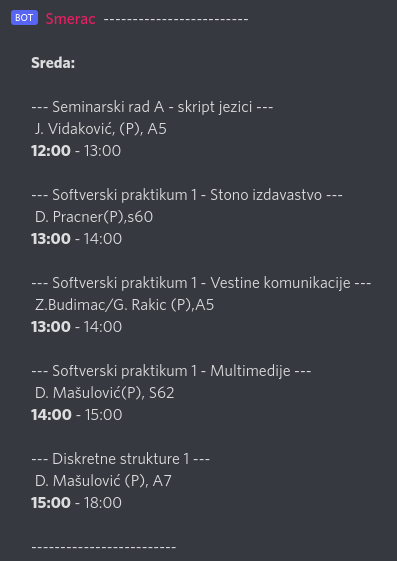
\includegraphics[height=8cm,width=5cm]{sreda} }}
    \hspace{1cm}
    \subfloat[Grafikon sa dnevnim prikazom časova, IT smer]{{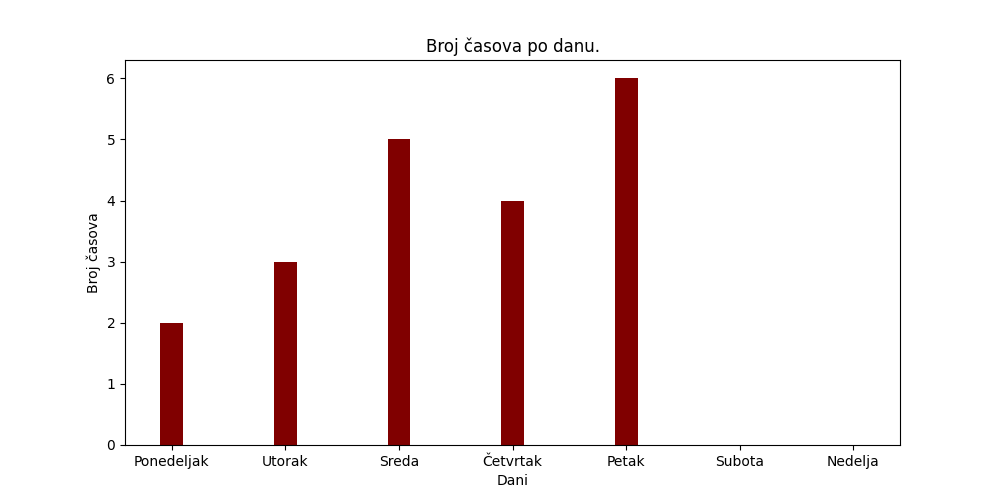
\includegraphics[height=5cm,width=7cm]{it} }}
    \hspace{1cm}
\end{figure}
\newpage

\section{Opis programa}
test
\newpage

\section{Zaključak}
test
\newpage

\pagestyle{plain}
\renewcommand\refname{Literatura}
\addcontentsline{toc}{section}{Literatura}
\bibliography{references}
\bibliographystyle{ieeetr}

\end{document}